\documentclass{article}

\usepackage{graphicx}
\usepackage{subcaption}
\usepackage{float}
\usepackage{enumitem}
\usepackage{hyperref}

\setlength{\parindent}{1.3em}
\setlength{\parskip}{0.7em}
\setlist{noitemsep}

\begin{document}

\begin{titlepage}
   \vspace*{\stretch{1.0}}
   \begin{center}
     \Huge\textbf{Vipassana for Hackers}\\
     \Huge{Paper Three: Why Meditate?}\\
     \vspace{5cm}
     \large\textit{Steven Deobald}\\
     \large\textit{Version 0.1 DRAFT}\\
     \large\textit\today\\
     \vspace{5cm}
     \large\textit{}\\
   \end{center}
   \vspace*{\stretch{2.0}}
\end{titlepage}

\begin{center}
  \Huge{Target Audience}
\end{center}

\textit{Vipassana for Hackers, Paper One: Curious Mechanics} was written to avoid discussing the
outcomes or consequences of meditation in detail. The focus of that paper was only
the internal mechanics of Vipassana meditation, to pique the interest of potential
meditators who had heard of Vipassana elsewhere. Outcomes are discussed only so far
as they assist the reader in understanding what is written earlier in the paper
regarding the senses. \textit{Paper Two: The Brain} goes further into the mechanics as they pertain to the
nervous system. Here, outcomes are discussed as they pertain to
neuroplasticity. Neither paper directly discusses why an individual might choose to
try this particular technique of meditation.

As before, the ``Hacker'' of \textit{Vipassana for Hackers} is not meant to identify
computer programmers. Instead, it is meant as a label for a culture of curious and
creative people who enjoy exploring, learning, and creating.

\textit{Paper Three: Why Meditate?} is written for anyone who has ever asked
themselves that very question or asked that question of their friends who
meditate. It is for both those who are curious about the practice of Vipassana
specifically and those who are curious about meditation in general. It is for people
who have meditated in other traditions and are curious about the benefits of
Vipassana. It is also for people who have never meditated in their entire lives. It
is intended for anyone who keeps hearing about Vipassana meditation --- in the media,
in books, and from friends --- and wants to learn what all the fuss is about.

The reader need not have read \textit{Paper One} or \textit{Paper Two}. In fact, it
is the intention of this paper to be the most accessible of the series and readers
with only a faint interest in the topic of meditation should start here.

\pagebreak

\begin{center}
  \Huge{Vipassana Basics}
\end{center}

Before we get to a discussion about why meditation is valuable, some basic
understanding of what meditation is (and isn't) is required.

The technique of Vipassana is based on a single underlying principle:

\vspace{1cm}
\textbf{Every experience which emerges in the mind, whether a thought, emotion, or contact of the five senses, always surfaces with a corresponding sensation on the body.}
\vspace{1cm}

It is important to understand this point as it underpins all other aspects of the
technique of Vipassana. Someone who is learning Vipassana need not accept this
principle as fact. Rather, a 10-day Vipassana course is a sort of laboratory where the
principle can be tested and experienced for oneself.

\begin{figure}[H]
  \centering
  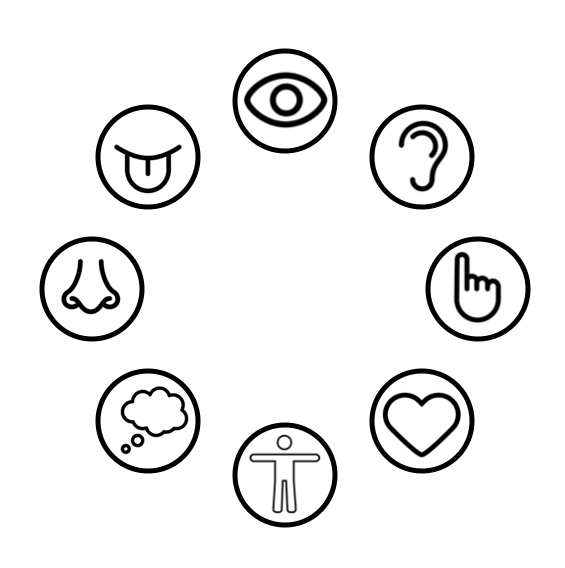
\includegraphics[width=11cm]{images/sense-doors.png}
  \caption{The sense doors and bodily sensation.}
  \label{fig:sense-doors}
\end{figure}

The totality of human experience can be categorized according to the ``sense doors''
listed in Figure~\ref{fig:sense-doors} \cite{sense-icons}: The five external sense doors of sight, sound,
taste, smell, and touch are listed at the top. The internal sense door of ``mind'' is
broken down into thought and emotion, second to the bottom. At the very bottom of the
diagram is bodily sensation, the object of meditation in Vipassana.

Once these eight experiences are listed, there is no experience left undescribed. All
human experience from the mundane (imagination, daydreaming, physical pleasures,
physical discomforts, etc.) to the supramundane (out-of-body experiences,
hallucinations, etc.) are subsets of these seven sense doors and their reflection in
bodily sensation, the eighth.

Mapping all of sensory experience to these eight categories begs the question of
attention, of awareness: Where does the meditator try to fasten her awareness? Where
is awareness normally? For the average person, awareness jumps around across these
eight categories. Even when one tries to focus on a difficult intellectual problem,
the discomforts of back pain and hunger or the distraction of an irritating sound
would draw attention away from thought, the desired object of attention. Vipassana
meditation asks the meditator to use bodily sensation as a gateway to the other seven
sense experiences. Rather than focusing on sound, focus on the sensation generated in
the body by the ear sense door. Rather than focusing on a thought or emotion, focus
on the sensation in the body generated by that thought or emotion. This is extremely
difficult to do, which is why (for lay people, in most cases) a 10-day silent
residential course \cite{dhamma} is necessary to learn the technique.

\begin{center}
  \Huge{The Mundane and The Supramundane}
\end{center}

Reasons for meditating will be broken down into two categories. \textit{The Mudane}
in this context refers not to the tedious but to the earthly, the material. Most people will begin
meditating for reasons in the mundane field simply because most people have never
experienced the supramundane. \textit{The Supramundane} in this context refers not to
spirituality or religion but experiences which transcend the material, physical
world.

Because supramundane experiences tend to occur only in deep meditative states,
the reasons for meditating listed will predominantly fall in the mundane
category. Whether or not the meditator experiences supramundane states in deep
meditation, these altered states of mind are never the goal of meditation. The goal
of meditation is to change the meditator's mental habits, to move away from unhealthy
mental patterns which cause harmful behaviours toward healthy mental patterns which
encourage productive behaviour. Obviously this change is only visible in the mundane
world, outside of meditation.

\begin{center}
  \Huge{Meditation vs. Naps}
\end{center}

While staying at a friend's house, I excused myself in the evening to meditate. He
sincerely asked, ``Is meditating for an hour really more valuable than using that
time for a good nap?''

\begin{itemize}
  \item posture
  \item sleep
  \item health (activation / motivation)
  \item ethics (activation / motivation)
  \item your children: a. knowing how to meditate, b. cross-legged posture
  \item emotion (i.e. anger)
  \item mundane sphere / productivity (21 lessons, seinfeld)
  \item reset frame of reference outside oneself, outside one's own lifetime: ``trees for god'' and obvious karma (sidu/booga smoking)
  \item unlearning obsessive / repetitive thought, enhancing creativity
  \item controlling unbounded sexuality without repression
  \item clarity: in thought, work, planning
  \item clarification: ``isn't that what makes us human?'' (emotions) --- rather, what makes us animal
  \item Die Standing Up

\end{itemize}

\pagebreak

\begin{thebibliography}{9}
\raggedright

\bibitem{sense-icons}
  5 Senses by Daniel Falk from the Noun Project
  \url{https://thenounproject.com/daniel2021/collection/human-body-senses/}
  Thought by Nociconist from the Noun Project
  \url{https://thenounproject.com/search/?q=thought&i=2025873}
  Heart by Rafael Garcia Motta from the Noun Project
  \url{https://thenounproject.com/search/?q=heart&i=807960}
  Body by Makarenko Andrey from the Noun Project
  \url{https://thenounproject.com/search/?q=body&i=789989}
  \textit{The Noun Project}.

\bibitem{dhamma}
  Vipassana International Academy
  \url{https://www.dhamma.org}
  \textit{Vipassana Meditation Website}


\end{thebibliography}

\end{document}
